\documentclass{report}
\usepackage[spanish]{babel}
\usepackage[utf8]{inputenc}
\usepackage{graphicx, longtable, float, titlesec, hyperref, enumitem, dingbat, multicol}
\usepackage[dvipsnames]{xcolor}
\usepackage[margin=2.75cm]{geometry}

\hypersetup{
    hidelinks = true
}

\titleformat{\chapter}[display]
  {\normalfont\bfseries}{}{0pt}{\Huge\thechapter.\space}

\titleformat{name=\chapter,numberless}[display]
  {\normalfont\bfseries}{}{0pt}{\Huge}

\titlespacing*{\chapter}{0pt}{-50pt}{20pt}

\begin{document}
    \begin{titlepage}
        \centering
        
\includegraphics[width=0.6\textwidth]{./img/logo.jpg}\\
        \vspace{1cm}
        \LARGE Software de Gestión de Empresa\\
        \vspace{0.5cm}
        \Large Ingeniería Informática de Gestión y Sistemas de Información\\
        \vspace{3cm}
        \Huge Proyecto de la asignatura\\
        \huge SoloG\\
        \vspace{2.5cm}
        \Large Autores:\\
        \vspace{0.2cm}
        \large Xabier Gabiña\\
        \large Ibai Sologuestoa\\
        \large Asier Cardoso\\
        \large Leire Becerra\\
        \large Adair Gondan\\
        \vfill
        \today
    \end{titlepage}
    \tableofcontents
    \listoffigures
    \listoftables
    \chapter{Análisis del sector}
      \paragraph*{}{El sector industrial de la videovigilancia es una parte de la industria de la seguridad y la tecnología. Se encarga de proporcionar sistemas de vigilancia visual para una amplia gama de aplicaciones en entornos industriales y domesticos, como fábricas, almacenes, instalaciones de energía, plantas de producción, hogares, entre otros.}
      \section{Productos ofertados}
        \paragraph*{}
        {
          Los productos ofertados en el sector de la videovigilancia son muy variados y se pueden clasificar en diferentes categorías. Algunos de los productos más comunes son: \cite{wiki-videovigilancia-ip}
        }
        \begin{multicols}{2}
          \begin{itemize}
            \item Cámaras de video
            \item Grabador de vídeo 
            \item Video Server Encoder
            \item Software de análisis de vídeo
            \item Dispositivos de visualización
            \item LED infrarrojos
            \item Sensores
            \item Reconocimiento Facial
          \end{itemize}
        \end{multicols}
        
      \section{Mercado objetivo}
        \paragraph*{}
        {
          El mercado objetivo de la videovigilancia es muy amplio y abarca desde la empresa hasta el hogar. 
          Aun así, el mayor volumen de ventas se da en el sector empresarial, donde se requieren sistemas de videovigilancia para proteger las instalaciones, controlar el acceso de personal y vehículos, y prevenir robos y actos vandálicos.
          Dentro del sector empresarial, se ha registrado un aumento en la demanda de sistemas de videovigilancia en el segmento de \textbf{infraestructuras críticas}, como aeropuertos, estaciones de tren, puertos, centrales eléctricas, entre otros.\cite{mordor-video-surveillance}
        }
        \paragraph*{}
        {
          Hay que tambien tener en cuenta que la demanda no es la misma en todos los países. La videovigilancia tiene un mayor peso en países como \textbf{Estados Unidos}, \textbf{China}, \textbf{Reino Unido}, \textbf{India} y \textbf{Brasil}, donde se han registrado un mayor número de instalaciones de sistemas de videovigilancia.\cite{mordor-video-surveillance}
        }
        \paragraph*{}
        {
          Tambien se espera que \textbf{Asia Pacífico} sea la región con mayor crecimiento en el mercado de la videovigilancia en los próximos años, debido al concepto de ciudades inteligentes ampliamente extendido especialmente en \textbf{China} y la creciente urbanización en la región.\cite{mordor-video-surveillance}
        }
        \begin{figure}[H]
          \centering
          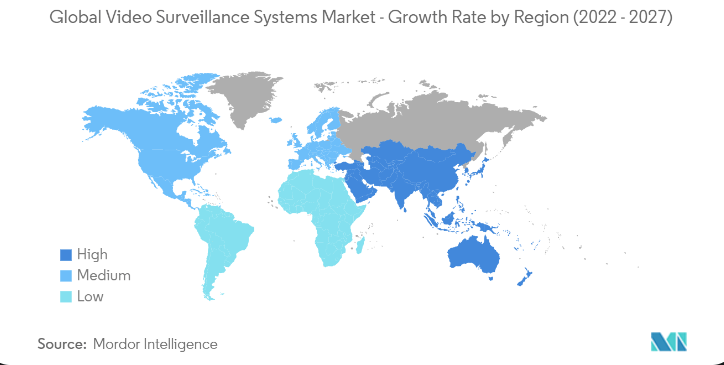
\includegraphics[width=0.7\textwidth]{./img/ssm.png}
          \caption{Mercado de la videovigilancia en 2022-2027}
        \end{figure}
      \section{Materias primas}
        \paragraph*{}{Las materias primas necesarias para la fabricación de los productos de videovigilancia son muchas y muy variadas. Algunas de las materias primas más usadas son:}
        \begin{multicols}{2}
          \begin{itemize}
            \item Plástico
            \item Metal
            \item Cables
            \item Circuitos integrados
            \item Lentes
            \item Sensores
            \item LED
            \item Software
          \end{itemize}
        \end{multicols}
      \section{Proveedores}
        \paragraph*{}
        {
          Los proveedores de materias para la fabricación de productos de videovigilancia se pueden clasificar en dos categorías, proveedores de componentes electrónicos y proveedores de software. 
          Algunos de los proveedores más importantes de componentes electrónicos son \textbf{Canon}, \textbf{Axis}, \textbf{Milestone} y \textbf{BCD}. 
          Algunos de los proveedores más importantes de software son \textbf{EarthCam} e \textbf{Infotech}
        }
      \section{Cinco fuerzas de Porter}
        \subsection*{Rivalidad entre competidores existentes}
          \paragraph*{}{El mercado de la videovigilancia es muy competitivo, con un gran número de empresas que ofrecen productos y servicios similares. La rivalidad entre competidores existentes es alta, lo que significa que las empresas deben competir en precio, calidad, innovación y servicio al cliente para mantener o aumentar su cuota de mercado.}
        \subsection*{Amenaza de productos sustitutos}
          \paragraph*{}{La amenaza de productos sustitutos en el mercado de la videovigilancia es baja, ya que los sistemas de videovigilancia son una parte esencial de la seguridad en muchos entornos, como empresas, hogares, infraestructuras críticas, entre otros.}
        \subsection*{Amenaza de productos o servicios sustitutos}
          \paragraph*{}{La amenaza de productos o servicios sustitutos en el mercado de la videovigilancia es baja, ya que los sistemas de videovigilancia son una parte esencial de la seguridad en muchos entornos, como empresas, hogares, infraestructuras críticas, entre otros.}
        \subsection*{Poder de negociación de los compradores}
          \paragraph*{}{El poder de negociación de los compradores en el mercado de la videovigilancia es alto, ya que los compradores tienen una amplia gama de opciones para elegir y pueden comparar precios, calidad, innovación y servicio al cliente antes de tomar una decisión de compra.}
        \subsection*{Poder de negociación de los proveedores}
          \paragraph*{}{El poder de negociación de los proveedores en el mercado de la videovigilancia es bajo, ya que hay muchos proveedores de componentes electrónicos y software que compiten por el negocio de las empresas de videovigilancia.}
      \section{Competidores}
        \paragraph*{}{Debido a que el mercado de la videovigilancia se actualiza constantemente los actores del mercado fluctuan mucho y son altamente competitivos. Los competidores más importantes en el mercado de la videovigilancia son:}
        \begin{multicols}{3}
          \begin{itemize}
            \item Axis Communications AB
            \item Bosch Security Systems Incorporated
            \item Honeywell Security Group
            \item Samsung Group
            \item Panasonic Corporation
            \item Schneider Electric SE
          \end{itemize}
        \end{multicols}
        \paragraph*{}{Como hemos comentado, el mercado de la videovigilancia es muy competitivo, lo que significa que \textbf{no es un mercado consolidado} por lo que se podria llegar a entrar y competir en el con una buena estrategia.}
        \begin{figure}[H]
          \centering
          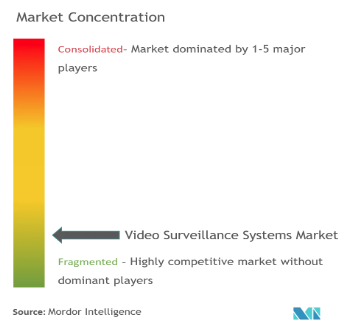
\includegraphics[width=0.4\textwidth]{./img/competidores.png}
          \caption{Competidores en el mercado de la videovigilancia}
        \end{figure}
    \chapter{Diseño del sistema de gestión}
        \section{Estructura empresarial} % Analizará el tipo de estructura organizacional, los departamentos y los diferentes niveles de decisión.
          \paragraph*{}
          {
            La estructura empresarial de SoloG es una estructura jerárquica, donde los empleados están organizados en diferentes departamentos y niveles de decisión. La estructura organizacional de SoloG se puede dividir en los siguientes departamentos:
          }
            \begin{multicols}{2}
              \begin{itemize}
                \item Dirección
                \item Administración
                \item Marketing
                \item Ventas
                \item Producción
                \item Logística
                \item Recursos Humanos
                \item I+D
              \end{itemize}
            \end{multicols}
          \paragraph*{}
          {
            Cada departamento tiene un gerente o jefe de departamento que es responsable de la gestión y coordinación de las actividades del departamento. Los gerentes de departamento informan al director general, que es el máximo responsable de la empresa y toma las decisiones estratégicas y de alto nivel.
            
          }
        \section{Procesos}
        \section{Usuarios}
    \chapter{Implementación de la solución}
    \chapter{Presentación de los resultados}
    \bibliographystyle{plain}
    \bibliography{bibliografia.bib}
\end{document}